\documentclass[../main.tex]{subfiles}
\begin{document}
Lo scripting in \code{bash} è utile per automatizzare compiti ripetitivi, combinando i comandi che abbiamo già visto e che da soli non 
sempre possono fare quello che ci serve.

Uno script è un file di testo che contiene dei comandi shell. Un file di questo tipo ha estensione \code{.sh} ma \underline{può anche
essere omessa}.

\textbf{Nota:} Bash è un \underline{linguaggio interpretato}. In caso di errori quindi lo script andrà avanti.

\vspace{0.5cm}
\subsection{Primi passi}
\begin{lstlisting}[style=bash]
    #!/bin/bash

    # Questo è un commento, e inizia con il cancelletto
    echo “Ciao mondo”
\end{lstlisting}
\begin{itemize}
    \item La prima linea di codice specifica che si sta utilizzando \code{bash}
    \item I commenti si fanno utilizzando il carattere \code{\#}
    \item Uno script può essere eseguito in due modi 
    \begin{itemize}
        \item \code{bash script.sh}
        \item \code{./script.sh} (solo con permessi di esecuzione)
        \item \code{script} (solo se lo script è nella directory \code{/bin}, accessibile solo da amministratore)
    \end{itemize}
\end{itemize}

\vspace{0.5cm}
\subsection{Variabili}
Le variabili possono essere solo \textbf{interi}, \textbf{stringhe}, o \textbf{array}, \code{bash} \underline{non supporta i numeri decimali}.
\begin{lstlisting}[style=bash]
    #!/bin/bash
    i=4
    x="ciao mondo"
    echo $x
\end{lstlisting}
\textbf{Nota:} non ci sono spazi intorno a \code{=}.

\textbf{Nota:} il carattere \code{\$} espande la variabile e ne restituisce il valore, questa operazione ha la precedenza sul globbing.
Per utilizzare invece il carattere '\$' si usa \code{\textbackslash\$} o si mette la stringa tra singoli apici.

\subsubsection{Variabili predefinite}
\begin{itemize}
    \item \code{\$0}, il nome dello script
    \item \code{\$1 .. \$n}, i parametri (per parametri > 10 usare \code{\$\{nn\}})
    \item \code{\$\#}, il numero dei parametri
    \item \code{\$@}, tutti i parametri (è un array)
    \item \code{\$\$}, il PID del processo della shell corrente
    \item \code{\$!}, il PID dell'ultimo processo mandato in background
    \item \code{\$?}, il valore di ritorno dell'ultimo comando eseguito (\code{0 = true}, altrimenti ha dato errore)
\end{itemize}
\textbf{Nota:} le variabili predefinite si possono sovrascrivere assegnando un altro valore.

\textbf{Nota:} con il comando \code{exit} si esce dallo script, possiamo specificare se il programma è andato a buon fine usando ad esempio
\code{exit 0} per la buona riuscita e \code{exit 1} per un uscita che ha generato errori.


\pagebreak
\subsection{Shift}
Il comando \code{shift} sposta i valori dei parametri posizionali
\begin{figure}[h]
    \centering
    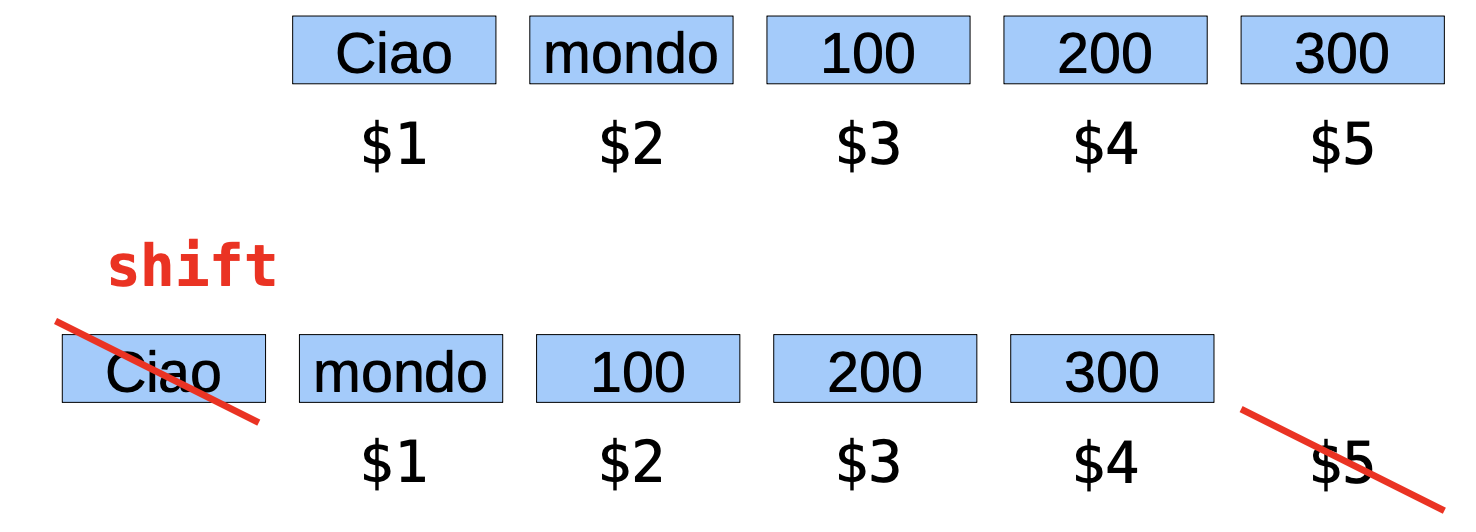
\includegraphics[width=0.7\textwidth]{../images/shift.png}
\end{figure}

\vspace{1cm}
\subsection{Read}
Il comando \code{read} legge l'input dell'utente e lo memorizza in una variabile
\begin{lstlisting}[style=bash]
    #!/bin/bash

    #Va a capo
    echo "Ciao come ti chiami?"
    read nome
    echo "Ciao $nome!"

    #Resta sulla riga corrente
    read -p “Come ti chiami?” nome
    echo “Ciao $nome!”

    #Resta sulla riga corrente e non mostra quello che l'untente inserisce da tastiera
    read -s -p “Password?” segreto
    echo “Conosco il tuo $segreto!”
\end{lstlisting}

\vspace{1cm}
\subsection{Catturare l'output di un comando}
Con \code{\$()} posso salvare \underline{l'output} di un comando in una variabile.
\begin{lstlisting}[style=bash]
    #!/bin/bash

    risultato=$(ls | grep "A") #Attennzione a non mettere spazi dove non servono

    echo "risultato: $risultato"
\end{lstlisting}

\pagebreak
\subsection{Test}
Per verificare una condizione si utilizza il comando \code{test}. Un'espressione vera (true) ritornerà \code{0} mentre un espressione falsa
ritornerà un valore diverso da zero.
\begin{lstlisting}[style=bash]
    #Equal
    test 5 -eq 5

    #Not equal
    [ 5 -ne 6 ] #Sintassi alternativa

    #Se la condizione è vera stampa 'OK'
    test 5 -eq 5 && echo "OK"
\end{lstlisting}
\begin{figure}[h]
    \centering
    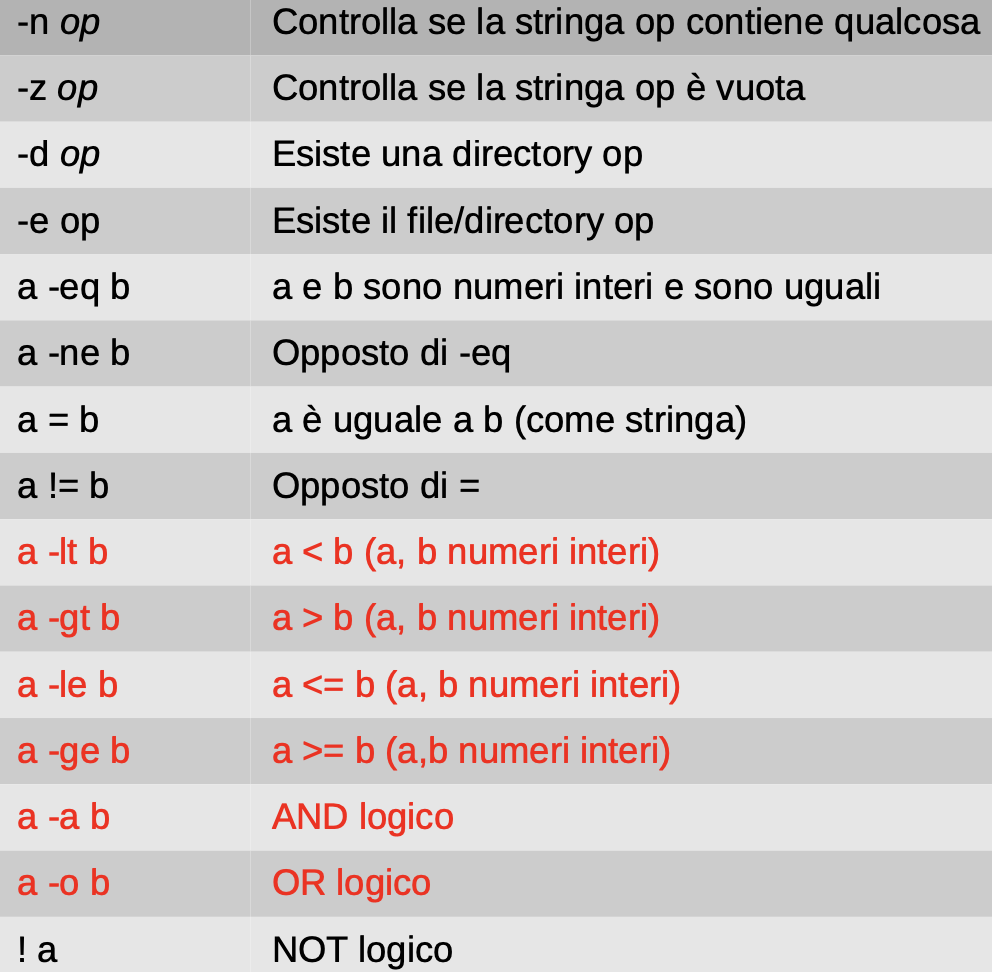
\includegraphics[width=0.6\textwidth]{../images/operatori.png}
\end{figure}

\vspace{0.25cm}
\subsubsection{Esempio}
Scriviamo uno script che accetta esattamente due parametri. Se il numero di parametri non è corretto termina l'esecuzione con un codice 
di errore, altrimenti scrive "OK"
\begin{lstlisting}[style=bash]
    ( test $# -eq 2 && echo "OK" && exit 0 ) || exit 1

    test $# -ne 2 && echo "errore" && exit 1
\end{lstlisting}
\textbf{Nota:} è importante lasciare uno spazio dopo la parentesi tonda.

\pagebreak
\subsection{Funzioni}
\begin{lstlisting}[style=bash]
    function saluta() {
        echo "Hello, world"
    }

    saluta
\end{lstlisting}
\textbf{Nota:} una funzione si usa con il suo nome senza l'aggiunta di parentesi tonde dopo.

\vspace{0.25cm}
\subsubsection{Esempio}
\begin{lstlisting}[style=bash]
    function somma() {
        echo $(expr $1 + $2)
    }

    somma 10 20
\end{lstlisting}

oppure utilizzando il \code{return}

\begin{lstlisting}[style=bash]
    function somma() {
        risultato=$(expr $1 + $2)
        return $risultato
    }

    echo $?
\end{lstlisting}
\textbf{Nota:} in questo caso \code{\$1} e \code{\$2} sono i parametri della funzione.

\vspace{1cm}
\subsection{Condizioni}
\begin{lstlisting}[style=bash]
    if mkdir nuovacartella 2>/dev/null; then
        echo "cartella creata"
    elif touch nuovofile 2>/dev/null; then
        echo "file creato"
    else
        echo "non posso creare ne cartella ne il file"
    fi
\end{lstlisting}
\textbf{Nota:} il comando \code{mkdir nuovacartella} restituisce \code{true} o \code{false} a dipendenza dell'esito del comando. La condizione
può essere un qualsiasi comando bash.

\vspace{0.25cm}
\subsubsection{Con \code{test}}
\begin{lstlisting}[style=bash]
    if [ $# -ne 2 ] && [ $1 -eq 5 ]; then
        echo "Devi passarmi due parametri e il primo deve essere 5"
        exit 1
    fi
    echo "tutto OK"
\end{lstlisting}

\begin{lstlisting}[style=bash]
    test=""

    if [ -n "$testo" ]; then
        echo "la stringa non è vuota"
    fi
\end{lstlisting}
\textbf{Nota:} usare sempre le virgolette quando si usa una variabile di testo.

\pagebreak
\subsection{Cicli}
\subsubsection{\code{while}}
\begin{lstlisting}[style=bash]
    i=1
    while [ $i -lt 10 ]; do
        echo "dentro il while, i vale: $i"

        i=$(expr $i + 1)
    done
\end{lstlisting}

\vspace{0.25cm}
Scorrere tutti i parametri (con \code{shift})
\begin{lstlisting}[style=bash]
    while [ $# -gt 0 ]; do
        echo "parametro: $1"
        shift
    done
\end{lstlisting}

\vspace{0.25cm}
Viene letto il contenuto del file dati.txt linea per linea
\begin{lstlisting}[style=bash]
    while read line; do
        echo "linea: $line"
    done < dati.txt
\end{lstlisting}

\vspace{0.5cm}
\subsubsection{\code{break} e \code{continue}}
\begin{lstlisting}[style=bash]
    while [ $# -gt 0 ]; do
        echo $1
        if [ "$1" = "x" ]; then
            break;
        fi
        shift
    done
\end{lstlisting}

\vspace{0.5cm}
\subsubsection{\code{for}}
Scorre tutti i parametri
\begin{lstlisting}[style=bash]
    for i in $@; do
        echo $i
    done
\end{lstlisting}

\vspace{0.25cm}
Scorre il contenuto di tutti file in base a un pattern
\begin{lstlisting}[style=bash]
    for file in $(ls /tmp); do
        while read linea; do
            echo "linea: $linea"
        done < $file
    done
\end{lstlisting}

\pagebreak
\subsubsection{\code{switch}}
\begin{lstlisting}[style=bash]
    for $file in *.txt; do
        case $file in
            a*) echo "inizia con a" ;;

            b*) echo "inizia con b" ;;

            *t*) echo "contiene una t" ;;

            *) echo "caso di default" ;;
        esac
    done
\end{lstlisting}

\end{document}